\documentclass[10pt,letterpaper,unboxed,cm]{article}
\usepackage[margin=1in]{geometry}
\usepackage{graphicx}
\usepackage{enumerate} 
\usepackage{amssymb} 
\usepackage{amsmath}
\usepackage{fancyhdr}
\usepackage{enumitem}
\usepackage{float}

\pagestyle{fancy}
\fancyhf{} 
\fancyhead[L]{CSE 105 Fall 2025}
\fancyhead[C]{Homework 3}
\fancyhead[R]{Due: Monday October 20 at 11:59pm}
\fancyfoot[L]{GROUP: Robin Villareal (A17450864), Tarun Upadhyay (A19113510), Kaitlyn Nguy (A19142421), Michelle Ho (A17326824)}
\fancyfoot[R]{\thepage} 

\begin{document}

\begin{enumerate}

\item \textbf{Converting an NFA to a DFA (Section 1)} \\
\emph{Question 1: Given the following NFA, create a DFA that recognizes the same language using subset construction by giving the final state diagram of the DFA.}

\begin{figure}[h]
    \centering
    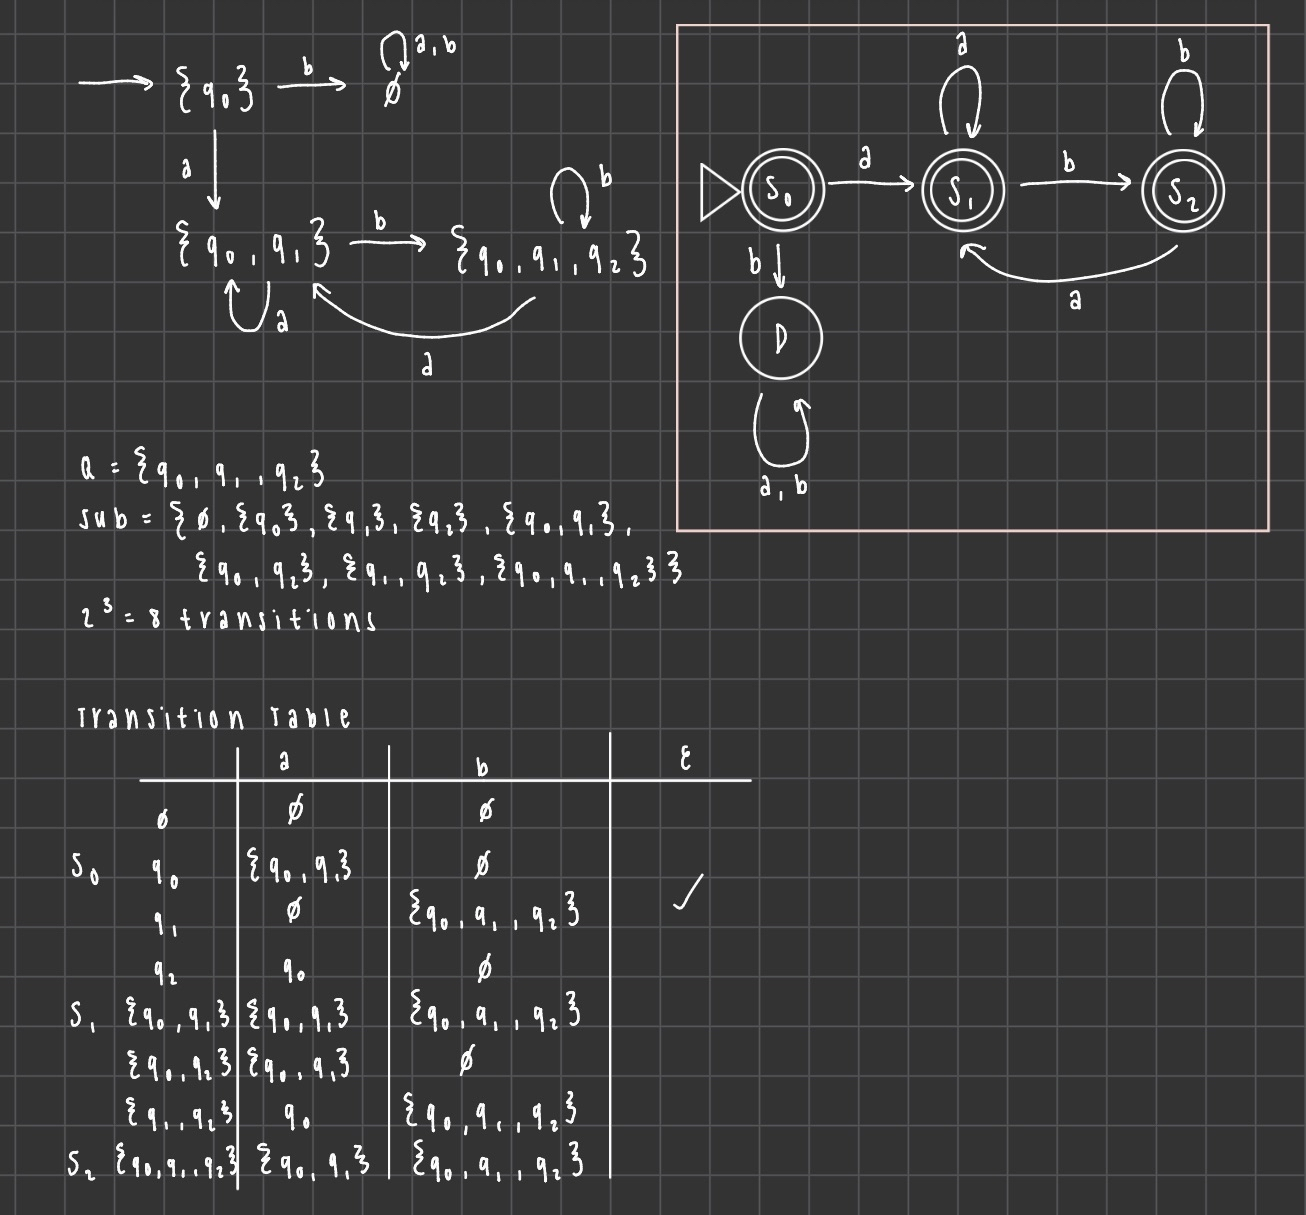
\includegraphics[width=1\linewidth]{hw3q1.png}
    \caption{Solution}
    \label{fig:placeholder}
\end{figure}

\pagebreak 

\item \textbf{Languages Described by Regular Expressions (Section 2)} \\
\emph{Question 5: Describe in words the language given by the regular expressions $R=1^*010^*$ over $\Sigma = \{0,1\}$ and 5 strings in the language and 5 strings not in the language.}

\textbf{Solution:}
\\$R=1^*010^*$ over $\Sigma=\{0,1\}$ describes the language $L$ over $\Sigma$ containing all the strings that have the substring "$01$" exactly once, that is preceded by 1's (could be zero 1's) and followed by 0's (possibly zero 0's).
\\\underline{Strings accepted:} \{"01", "1101", "010", "1010", "11010"\}
\\\underline{Strings not accepted:} \{"", "1", "0", "10", "111000"\}

\pagebreak

\item \textbf{Converting from Regular Expressions (Section 3)} \\
\emph{Question 10: Create an NFA that recognizes the same language as $L(((11)^*0^*1)\cup((00)^*1^*0)^*)$ over $\Sigma=\{0,1\}$.}

\begin{figure}[h]
    \centering
    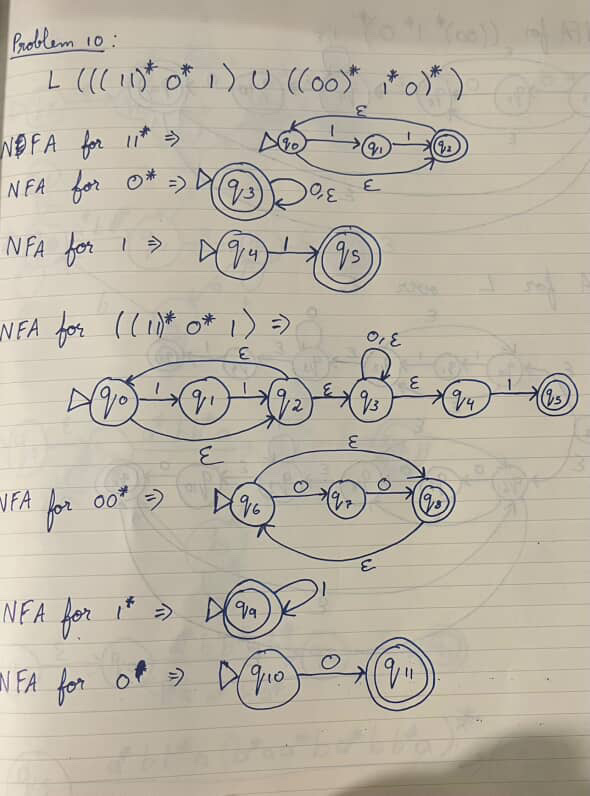
\includegraphics[width=0.75\linewidth]{hw3q10p1.jpg}
    \caption{Solution pt. 1}
    \label{fig:placeholder}
\end{figure}

\pagebreak

\begin{figure}[h]
    \centering
    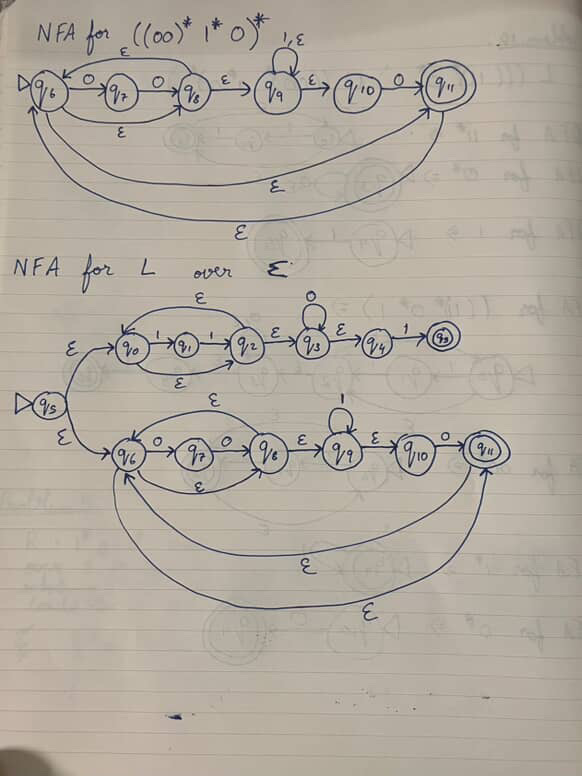
\includegraphics[width=0.75\linewidth]{hw3q10p2.jpg}
    \caption{Solution pt. 2}
    \label{fig:placeholder}
\end{figure}

\pagebreak 

\item \textbf{Converting from Automata to Regular Expressions (Section 4)} \\
\emph{Question 13: Given the DFA $D$ and $D$'s state diagram given below, find the regular expression $R$ such that $L(R)=L(D)$ by constructing a GNFA. Give all of the steps of your GNFA construction alongside $R$.}

% Add your answer content here

\pagebreak

\item \textbf{Proving Closure of Regular Operations Using Regular Expressions (Section 5)} \\
\emph{Question 17: Given a regular language $L$, recall that the reversal of the language is denoted as $L^R$, and it is the language of all the strings in $L$, but they are reversed. Given any regular expression $R$, prove that $L(R)^R$ is regular by constructing a regular expression $R^R$ such that $L(R^R) = L(R)^R$.}

% Add your answer content here

\end{enumerate}

\end{document}
